%---------------------------------------------------------------------------%
%-                                                                         -%
%-                           LaTeX Template                                -%
%-                                                                         -%
%---------------------------------------------------------------------------%
%- Copyright (C) Huangrui Mo <huangrui.mo@gmail.com>
%- This is free software: you can redistribute it and/or modify it
%- under the terms of the GNU General Public License as published by
%- the Free Software Foundation, either version 3 of the License, or
%- (at your option) any later version.
%---------------------------------------------------------------------------%
%->> Document class declaration
%---------------------------------------------------------------------------%
\documentclass[printcopy,fontset=windows]{Style/neuthesis}%
%- Multiple optional arguments:
%- [<singlesided|doublesided|printcopy>]% set one or two sided eprint or print
%- [draftversion]% show draft version information
%- [fontset=<fandol|windows|mac|adobe>]% specify font set to replace automatic detection
%- [scheme=plain]% thesis writing of international students
%- [standard options for ctex book class: draft|paper size|font size|...]%
%---------------------------------------------------------------------------%
%->> Document settings
%---------------------------------------------------------------------------%
\usepackage[toc]{appendix}
\usepackage[export]{adjustbox}% set the max width of graphics
\usepackage{rotating}% Use "sidewaystables" to rotate images. Includes "graphicx" automatically
\usepackage{longtable}% A kind of table that can be split into multiple pages
\usepackage[bibtex,myhdr,table,list,geometry]{Style/artratex}
% document settings
%- usage: \usepackage[option1,option2,...,optionN]{artratex}
%- Multiple optional arguments:
%- [bibtex|biber]% set bibliography processor and package
%- [geometry]% reconfigure page layout via geometry package
%- [lscape]% provide landscape layout environment
%- [myhdr]% enable header and footer via fancyhdr package
%- [color]% provide color support via xcolor package
%- [background]% enable page background
%- [tikz]% provide complex diagrams via tikz package
%- [table]% provide complex tables via ctable package
%- [list]% provide enhanced list environments for algorithm and coding
%- [math]% enable some extra math packages
\usepackage{Style/artracom}% user defined commands
\usepackage{emptypage}
%---------------------------------------------------------------------------%
%->> Document inclusion
%---------------------------------------------------------------------------%
%\includeonly{Tex/Chap_1,...,Tex/Chap_N}% selected files compilation
%---------------------------------------------------------------------------%
%->> Document content
%---------------------------------------------------------------------------%
\def\alltex{}
\begin{document}
% \layout
%-
%-> Frontmatter: title page, abstract, content list, symbol list, preface
%-
\frontmatter% initialize the environment
% !TEX ROOT = ../Thesis.tex 
%---------------------------------------------------------------------------%
%->> 封面信息及生成
%---------------------------------------------------------------------------%
%-
%-> 中文封面信息
%-
\category{}%分类号
\confidential{}% 密级:只有涉密论文才填写
\UDC{}
\schoollogo% 校徽
% \schooltitle{width=1cm}{neu_title}
\title{这是一个标题\vspace{10pt}的第二行}% 论文中文题目
\subtitle{}
\author{某某某}% 论文作者
\advisor{某 某 \quad 教授}% 指导教师:姓名 专业技术职务 工作单位
\advisorsec{某某某 \quad 工程师}% 指导老师附加信息 或 第二指导老师信息
\degree{学士}% 学位:学士、硕士、博士
\degreetype{工学}% 学位类别:理学、工学、工程、医学等
\major{信息安全}% 二级学科专业名称
\institute{软件学院}% 院系名称

\research{}% 研究方向
\authorno{20170000}% 学号
\chinesedate{2021~年~6~月}%  封面页脚日期
\submissiondate{2021~年~6~月}% 论文提交日期
\oraldefencedate{2021~年~6~月}% 论文答辩日期
\degreedate{2021~年~6~月}% 学位授予日期
\chairman{某某某}% 答辩委员会主席
%-
%-> 英文封面信息
%-
\englishtitle{Design and Implementation of an \vspace{10pt} XXX Based \vspace{10pt} XXX}% 论文英文题目
\englishauthor{\vspace{-20pt}Mou Moumou}% 论文作者
\englishadvisor{Professor \quad Mou Mou}% 指导教师
\englishadvisorsec{Engineer \qquad \qquad \quad \hspace{0.58mm} Mou Moumou} % 第二指导教师
\englishdegree{Bachelor}% 学位:Bachelor, Master, Doctor。封面格式将根据英文学位名称自动切换,请确保拼写准确无误
\englishdegreetype{Engineering}% 学位类别:Philosophy, Natural Science, Engineering, Economics, Agriculture 等
\englishthesistype{thesis}% 论文类型: thesis, dissertation
\englishuniversity{Northeastern University}
\englishmajor{}% 二级学科专业名称
\englishinstitute{Software College}% 院系名称
\englishdate{June 2021}% 毕业日期:春季 April 夏季为June、秋季为September 冬季为December
%-
%-> 生成封面
%-
%\makereviewcover % 生成盲审中文封面
\makeprintcover %生成打印的中文封面
\makeenglishtitle% 生成英文页
\makechinesetitle % 生成中文内容页
%-
%-> 作者声明
%-
\makedeclaration% 生成声明页
% title page, abstract, dedication
% !TEX ROOT = ../Thesis.tex 

%-
%-> 英文摘要
%-
\chapter{\bf{ABSTRACT}}\chaptermark{Abstract}% 摘要标题

This is the abstract.

\englishkeywords{This; Abstract}

%-
%-> 中文摘要
%-
\chapter[摘\quad 要]{摘\quad 要}\chaptermark{摘要}% 摘要标题
% \setcounter{page}{1}% 开始页码
% \pagenumbering{Roman}% 页码符号
% 22p / 12p = 1.83
\linespread{1.5}
\zihao{-4}
% \setlength{\baselineskip}{20pt}

这是一个摘要。

\vspace{-3pt}新的一段。

\keywords{这;摘要}% 中文关键词

 % abstract (chinese and english)

{% content list region
% \linespread{1}
% \intotoc{\contentsname}% add link to contents table and bookmark
% \chapter*{\contentsname}
\linespread{1.5}% local line space
\tableofcontents% contents catalog
\markboth{Content}{Content}

%\intotoc{\listfigurename}% add link to contents table and bookmark
%\listoffigures% figures catalog

%\intotoc{\listtablename}% add link to contents table and bookmark
%\listoftables% tables catalog
}
% \input{Tex/Prematter}% list of symbols, preface content
%-
%-> Mainmatter
%-
\mainmatter% initialize the environment
\linespread{1.4}
\zihao{-4}
%---------------------------------------------------------------------------%
%->> Main content
%---------------------------------------------------------------------------%
\chapter{Introduction}\label{chap:introduction}

\section{Research Background}

This is the research background.

\begin{table}[!htbp]
	\setlength{\abovecaptionskip}{0cm}%  
	\setlength{\belowcaptionskip}{-0.1cm}%设置表名与表间距离
	\caption{Layers of a blockchain system}
	\centering
	\begin{small}
	\begin{tabular}{l l}
		\Xhline{1.5pt}
		{\bfseries Layer} & {\bfseries Sublayer} \\
		\Xhline{1.5pt}
		Application layer & \\ \hline
		\multirow{2}{*}{Smart contract layer} & Programming language \\ \cline{2-2}
		& Sandbox environment \\ \hline
		\multirow{3}{*}{Data layer} & Data structures \\ \cline{2-2}
		& Data models \\ \cline{2-2}
		& Data storage \\ \hline
		Consensus layer & \\ \hline
		Network layer & \\
		\Xhline{1.5pt}
	\end{tabular}
	\end{small}
\end{table}

This is the research background.

\section{Research Significance}
This is the research significance.

\begin{enumerate}
	\item A.
	\item B.
	\item C.
	\item D.
\end{enumerate}

\section{Thesis Organization}
This paper is organized as follows:

\textbf{Chapter 1:} Introduction, research background, research significance, research status, research contents and the organizational structure of the paper have been introduced in this chapter.

\textbf{Chapter 2:} System design. How the modules are composed and how the partitions are layered will be presented. The reasons of such designs and what problems they can solve will be explained.

\textbf{Chapter 3:} Summary and future work. A brief summary of the work and plans for the follow-up work.


\definecolor{dkgreen}{rgb}{0,0.6,0}
\definecolor{gray}{rgb}{0.5,0.5,0.5}
\definecolor{mauve}{rgb}{0.58,0,0.82}
\lstset{frame=tb,
	language=Java,
	aboveskip=3mm,
	belowskip=3mm,
	showstringspaces=false,
	columns=flexible,
	basicstyle=\rmfamily\fontsize{10.5pt}{12.6pt}\selectfont,
	numbers=none,
	numberstyle=\tiny\color{gray},
	keywordstyle=\color{blue},
	commentstyle=\color{dkgreen},
	stringstyle=\color{mauve},
	breaklines=true,
	breakatwhitespace=true,
	tabsize=3
}
\chapter{System Design} \label{chap:system-design}

\section{Design Overview}
In this section, the overview design of the system is described.

\subsection{Architecture Design}

This is the Architecture Design.

\begin{figure}[!h]
	\centering
	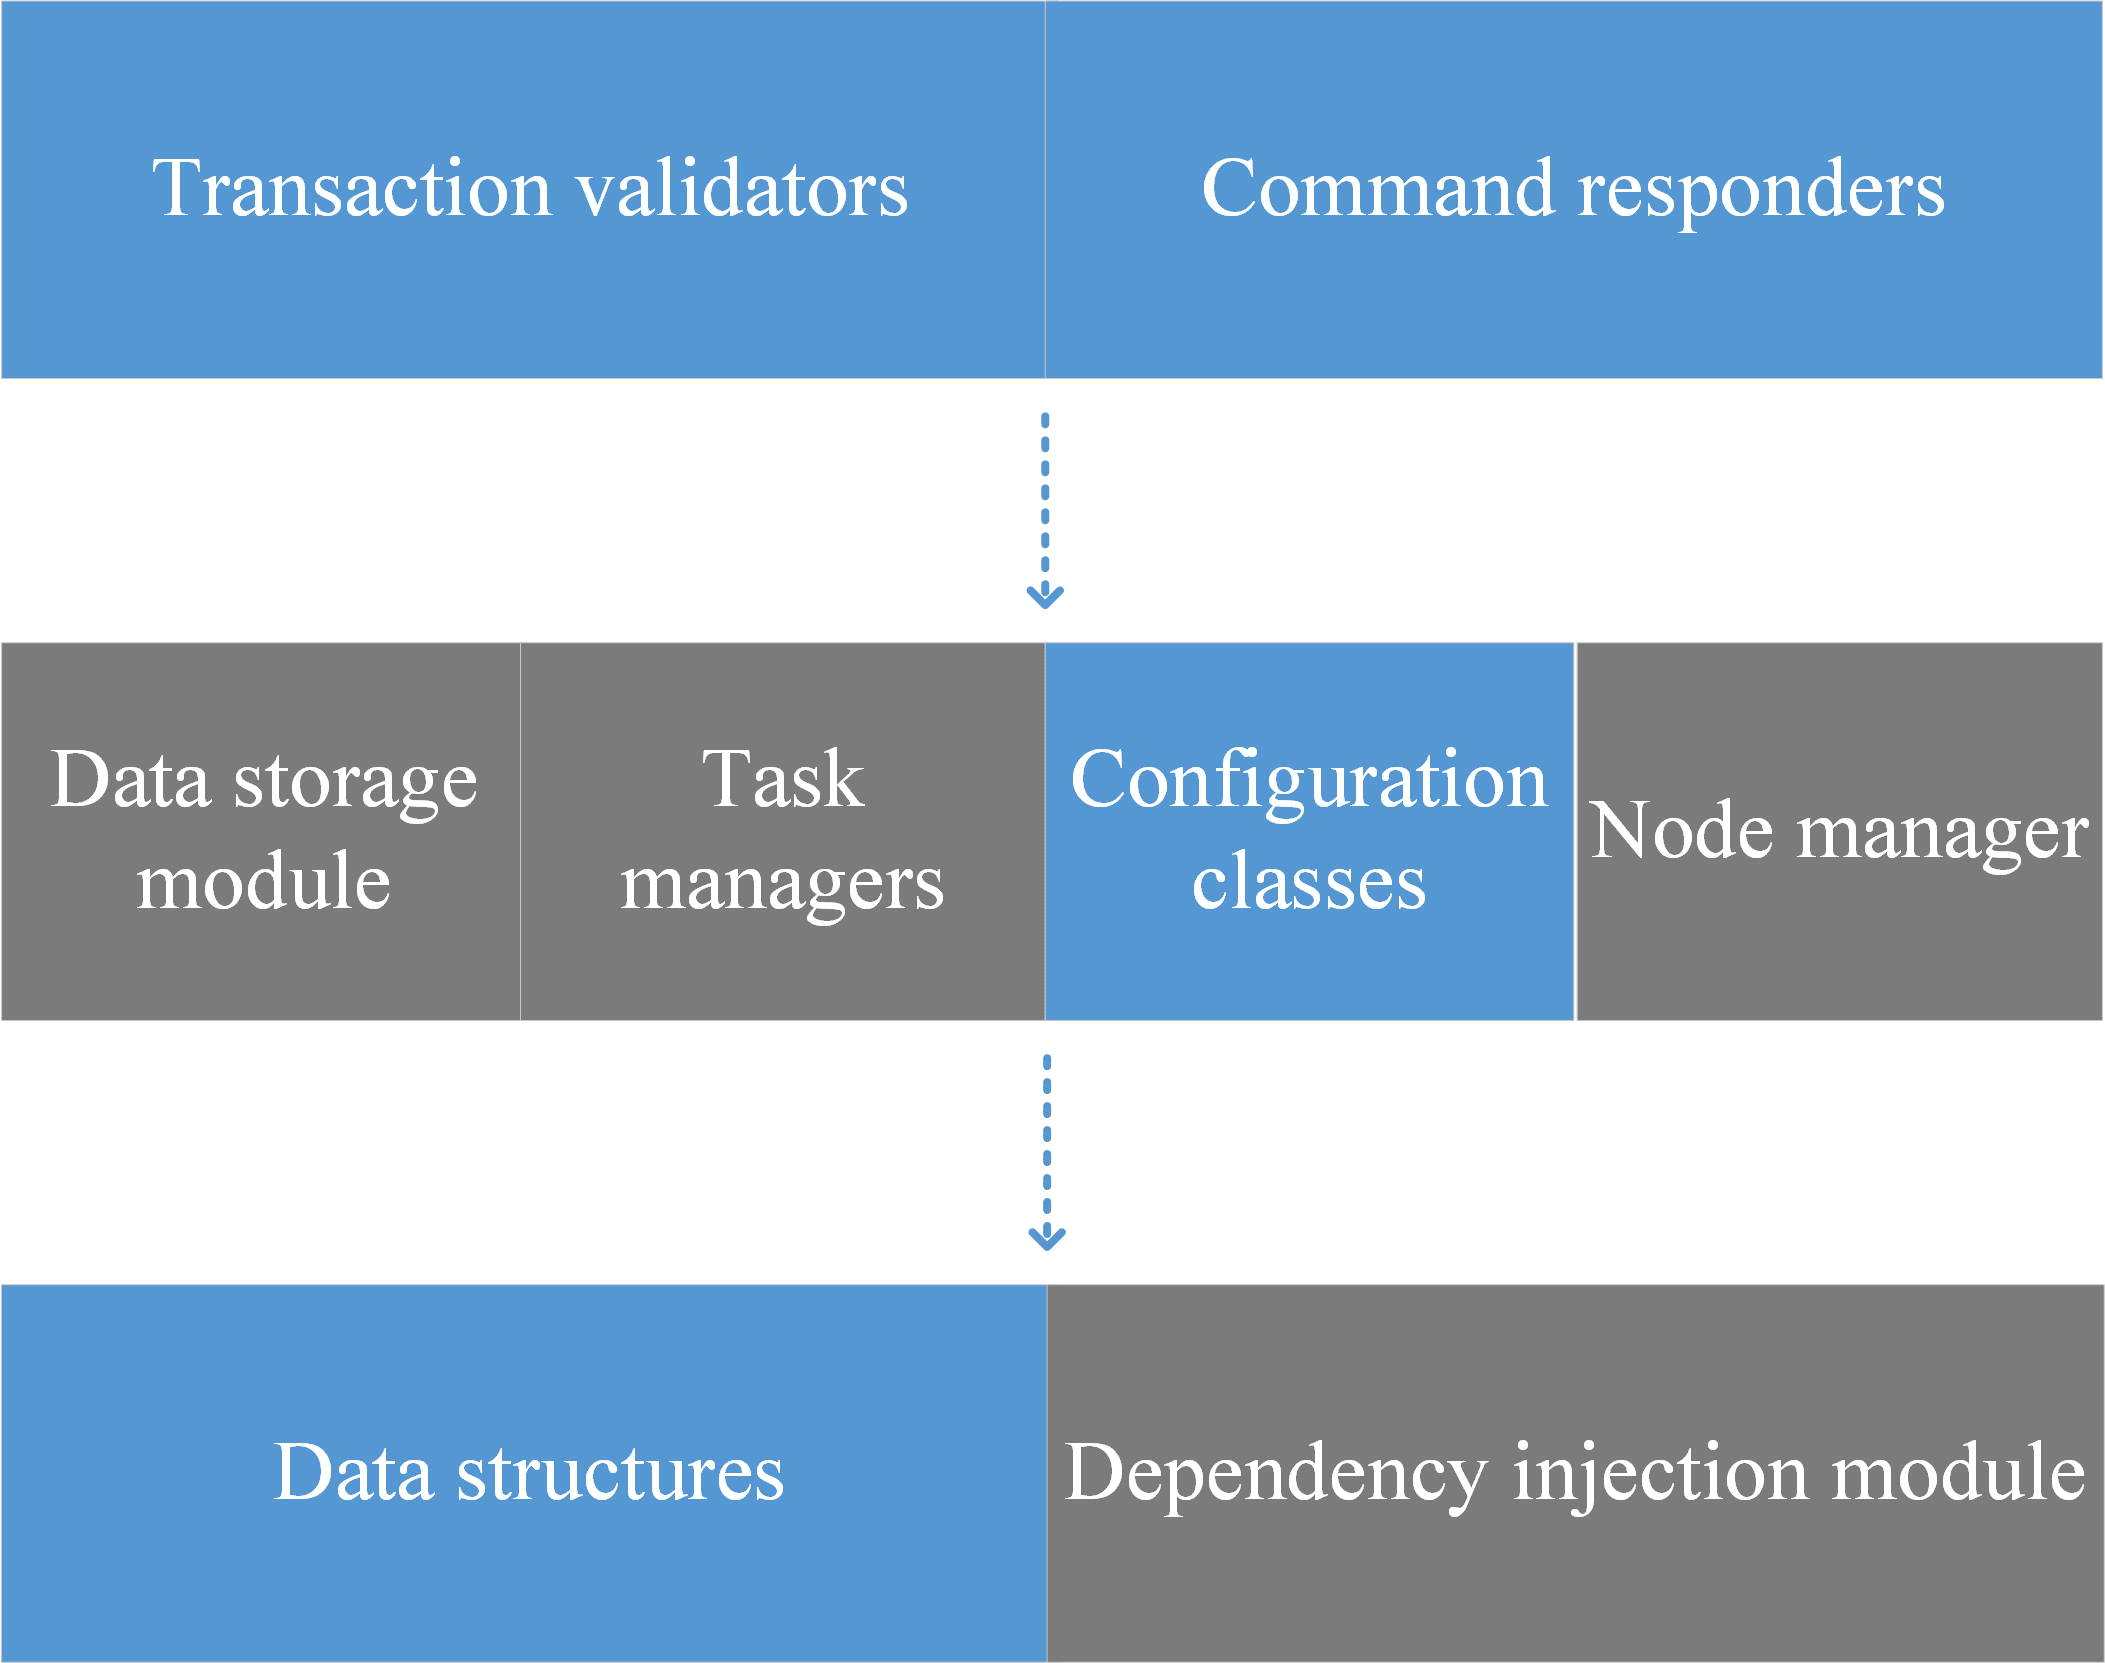
\includegraphics[width=0.65\textwidth]{Architecture_Sketch_Map}
	\caption{Architecture sketch map}
	\label{fig:architecture-sketch-map}
\end{figure}

\subsection{Module Design}

This is the Module Design.

\begin{figure}[!htbp]
	\centering
	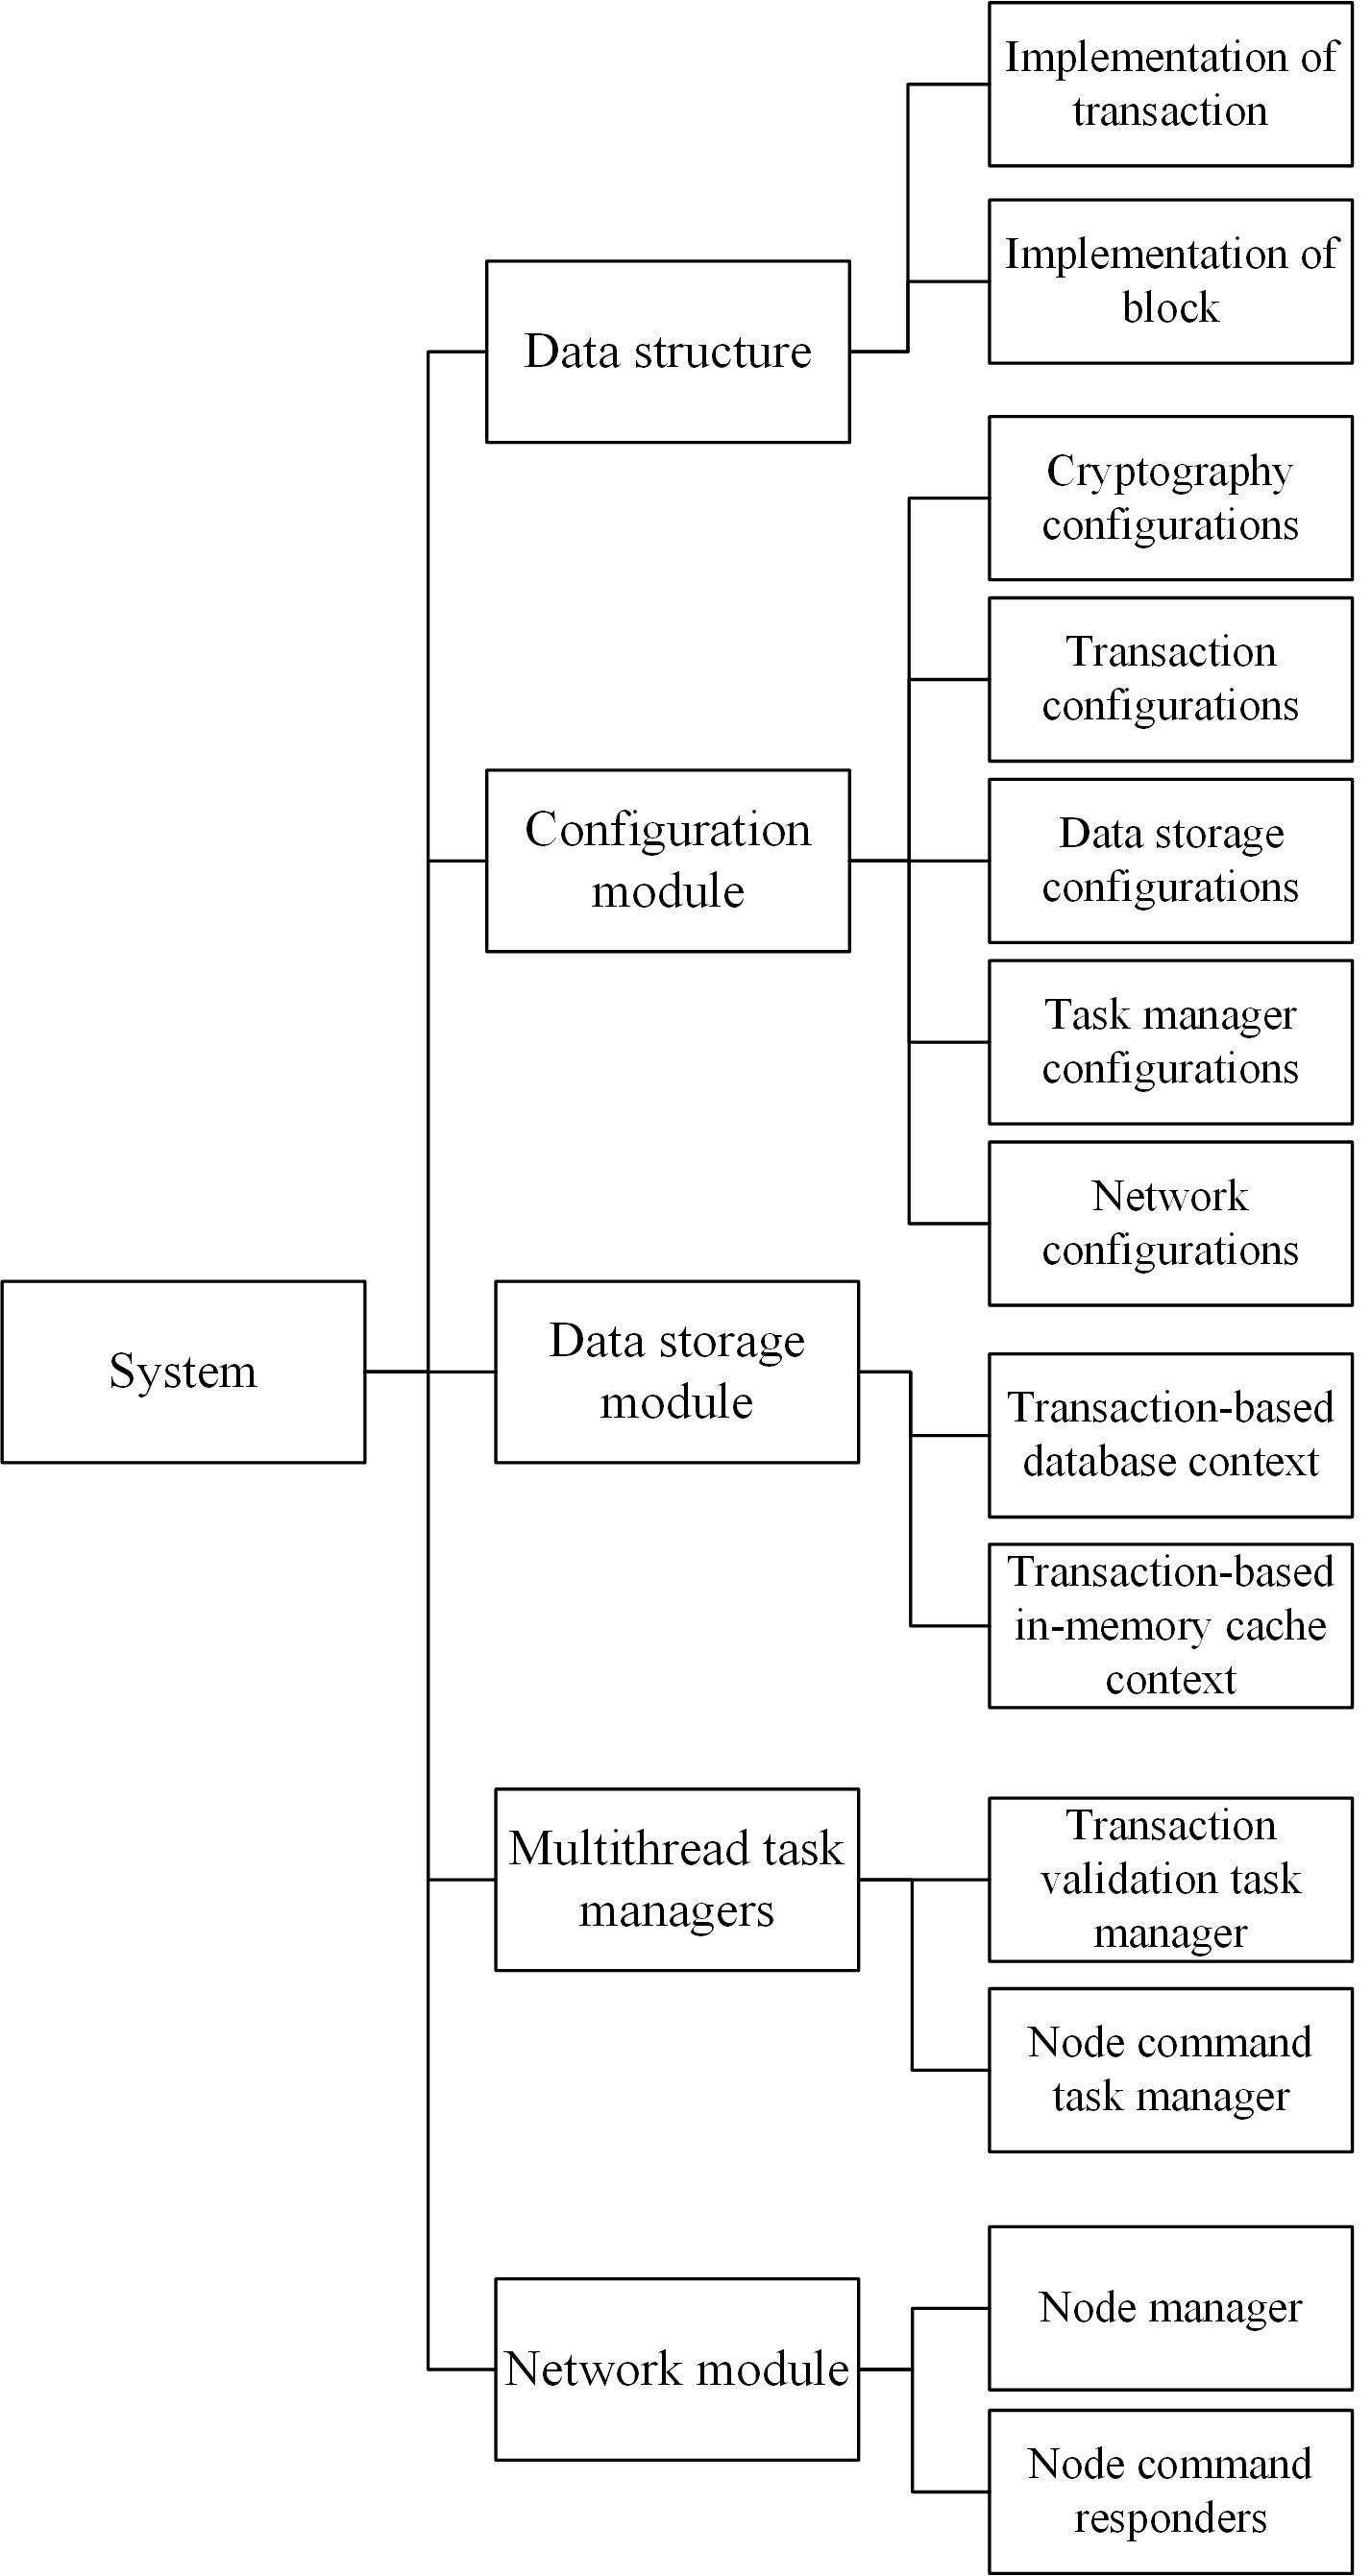
\includegraphics[max width=0.6\textwidth]{Module_Design_(Integrated,_Modules_Evenly_Distributed)}
	\caption{Module design sketch map}
	\label{fig:module-design}
\end{figure}

% \section{Detailed Design}\label{sec:system-design:detailed-design}
% In this section, the detailed design of the system is presented, following the order of module division mentioned above.

\subsection{Data Structure}

\begin{table}[!htbp]
\setlength{\abovecaptionskip}{0cm}%  
\setlength{\belowcaptionskip}{-0.1cm}%设置表名与表间距离
\centering
\caption{Data structure of a block in Bitcoin}
\label{tab:block_in_bitcoin}
 
\begin{small}
	\begin{tabular}{l l}
		\Xhline{1.5pt}
		{\bfseries Field} & {\bfseries Purpose} \\
		\Xhline{1.5pt}
		version & Version of the block \\
		\hline
		hashPrevBlock & Hash of the previous block \\
		\hline
		hashMerkleRoot & Hash of Merkle root; for indexing transactions and ensuring validity of them \\
		\hline
		time & Unix epoch in UTC \\
		\hline
		bits & Contains info about the hash target of PoW or interpreted as the difficulty \\
		\hline
		nonce & A random number; involved in hash generation of the block \\
		\hline
		transactions & Transactions included in the block \\
		\Xhline{1.5pt}
	\end{tabular}
\end{small}
\end{table}

\section{Summary}
This chapter demonstrates the overall architecture and more detailed designs including the data structures, several modules and the general startup procedures. Some contents have been described as to what design pattern can be used and how extensions can be built using the interfaces. They will guide the implementations in the next chapter.


\chapter{Conclusion and Future Work}
This is the Conclusion and Future Work.

\section{Conclusion}
This is the Conclusion.

% \input{Tex/Chap_Guide}
%---------------------------------------------------------------------------%
% main content

% \layout
%-P

%-
%-> Backmatter: bibliography, glossary, index
%-
\backmatter% initialize the environment
\intotoc{\bibname}% add link to contents table and bookmark
\bibliography{Biblio/ref}% bibliography
\makereference
\nocite{*} % temprorarily allow nocite

\appendix
\chapter{Appendix}
这是一个附录。


\chapter[Acknowledgement]{Acknowledgement}\chaptermark{Acknowledgement}% syntax: \chapter[目录]{标题}\chaptermark{页眉}
% \thispagestyle{noheaderstyle}% 如果需要移除当前页的页眉
%\pagestyle{noheaderstyle}% 如果需要移除整章的页眉

\reviewORprint{
}{
This is the acknowledgment.
}

%\chapter{攻读博士学位期间取得的学术成果}

%\section*{个人简历:}


%\reviewORprint{
    %\section*{第一作者发表/录用学术论文:}
    %\begin{enumerate}[leftmargin=*]
        %\item Title[J]Journal, Year, Volume(Number):Pages. (\textbf{SCI, JCR1, 论文第三章})
    %\end{enumerate}
    %\section*{第一作者在审学术论文:}
    %\begin{enumerate}[leftmargin=*]
        %\item Title[J]Journal, Year, Volume(Number):Pages. (\textbf{SCI, JCR1, 论文第三章})
    %\end{enumerate}
    %\section*{通讯作者发表/录用学术论文:}
    %\begin{enumerate}[leftmargin=*]
        %\item Title[J]Journal, Year, Volume(Number):Pages. (\textbf{SCI, JCR1, 第二作者/通讯作者})
    %\end{enumerate}
    %\section*{合作作者发表/录用学术论文:}
    %\begin{enumerate}[leftmargin=*]
        %\item Title[J]Journal, Year, Volume(Number):Pages. (\textbf{SCI, JCR1, 第二作者})
    %\end{enumerate}
%}{
    %\section*{学术论文:}
    %\begin{enumerate}[leftmargin=*]
        %\item Authors. Title[J]Journal, Year, Volume(Number):Pages.
    %\end{enumerate}
%}

%\section*{科研项目:}

%\begin{enumerate}[leftmargin=*]
    %\item 项目类型,项目号, 项目名称, 日期。
%\end{enumerate}

\cleardoublepage% 让文档总是结束于偶数页,可根据需要设定页眉页脚样式,如 [noheaderstyle]

% other information
% \showthe\artxfontset
\end{document}
%---------------------------------------------------------------------------%

